\chapter{Transition: Final Release and Validation}
\label{chap:transition}

\section{Introduction}

The transition phase delivers the system to its users. This chapter presents the final release use case by use case, the test strategy and its results, the traceability of the requirements, the installation and documentation of the platform, and the scope within which it can be considered stable.

\section{Final application tour}
\label{sec:tour}

The screenshots below show the final release during the analysis of the Jaguar I-PACE holdout recording, a file the Jaguar I-PACE model never saw during its training. The title bar shows the short name of the application, CANvision.

\begin{itemize}
    \item \textbf{Import log:} Every session starts on the Home screen, with the choice between a live session and an offline import (Figure~\ref{fig:screen-home}). The live session stays locked until the backend runs and a USB adapter, such as an Arduino board, is plugged in. Importing a log leads to the choice of the vehicle model, with the status of each model.
\end{itemize}

\begin{figure}[H]
\centering
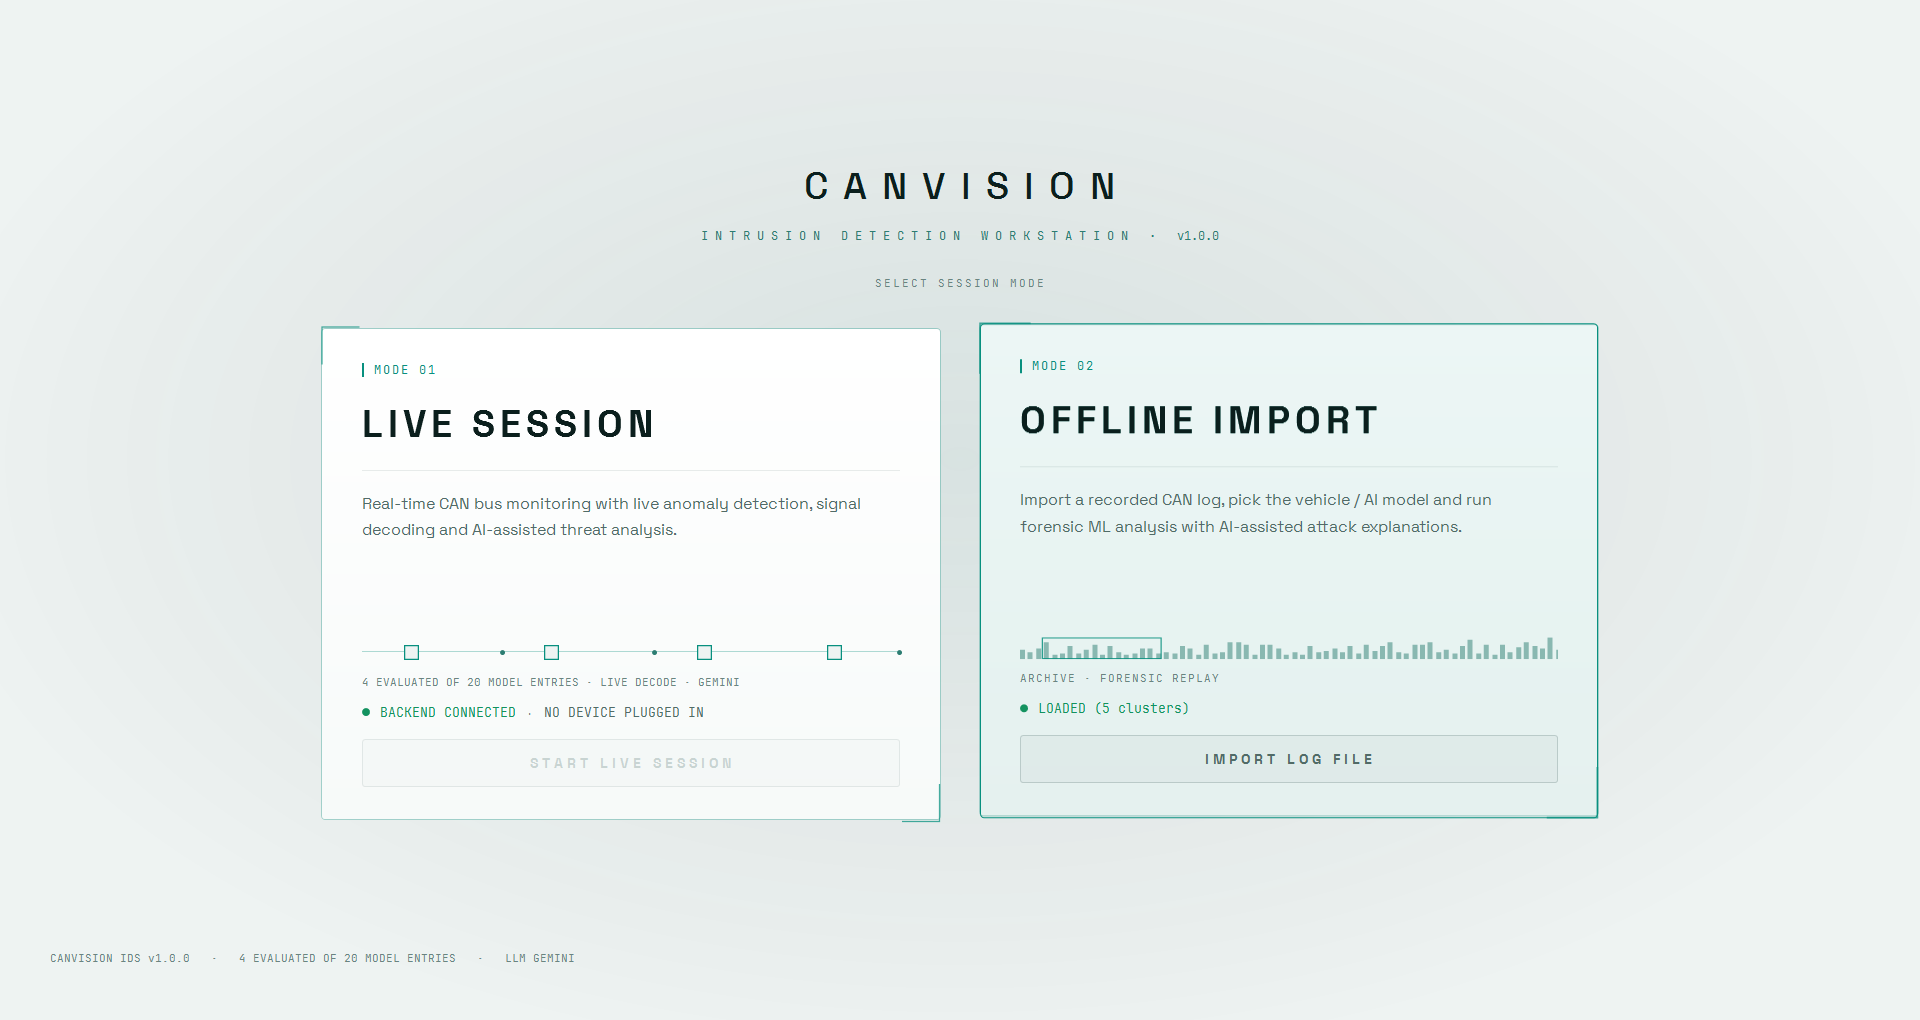
\includegraphics[width=0.72\textwidth]{f01_home.png}
\caption{Home screen: choice between a live session and an offline import.}
\label{fig:screen-home}
\end{figure}

\begin{itemize}
    \item \textbf{Detect anomaly and review the results:} After the analysis, the Dashboard (Figure~\ref{fig:screen-dashboard-final}) shows the highest flagged score, the number of alerts, the share of scored frames that were flagged, the unresolved frames with their reasons, the trend of the scores and the bus monitor. For this file, the application read 50{,}361 frames, scored 40{,}477 and flagged 1{,}249, the 3.09\% of Table~\ref{tab:holdout-results}, with flagged scores from 0.500 to 0.935 and 339 alerts after the merging of bursts.
\end{itemize}

\begin{figure}[H]
\centering
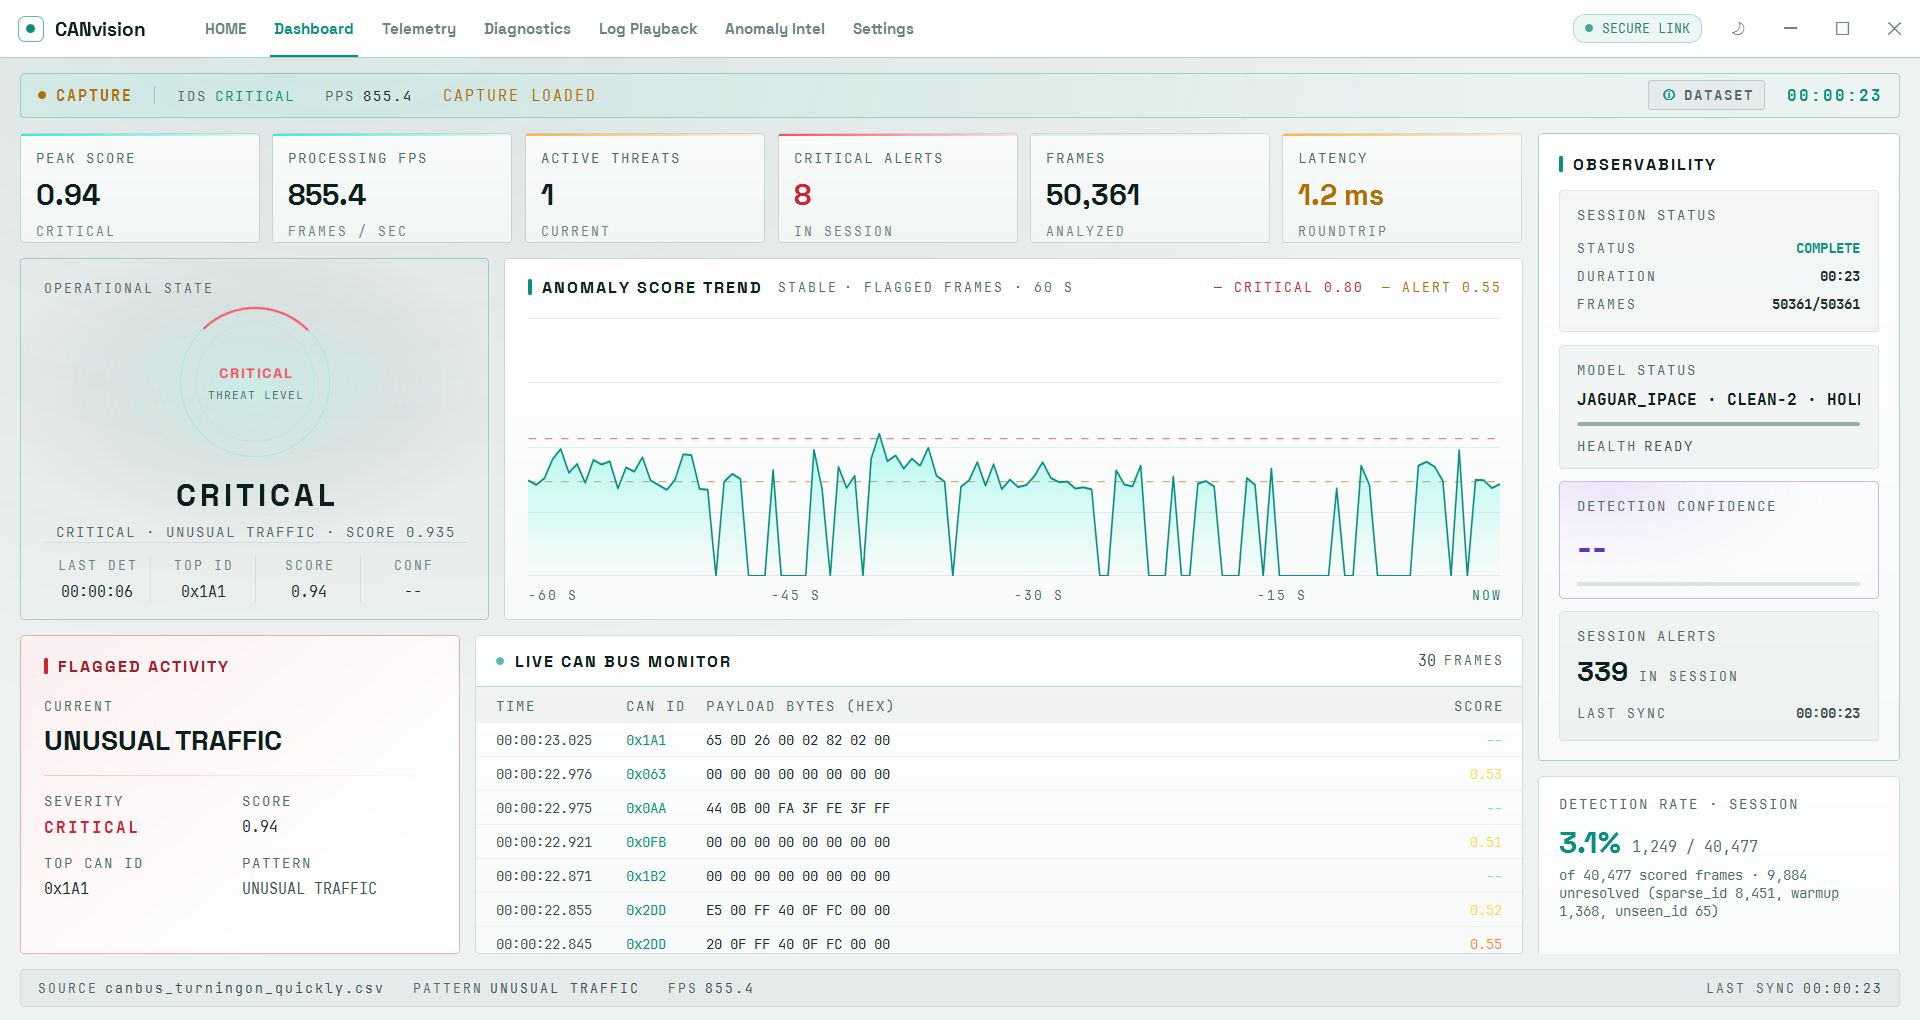
\includegraphics[width=\textwidth]{f02_dashboard.png}
\caption{Dashboard after the analysis of the Jaguar I-PACE holdout recording.}
\label{fig:screen-dashboard-final}
\end{figure}

\begin{itemize}
    \item \textbf{Describe capture:} The Dataset button opens a card that describes the recording in plain words (Figure~\ref{fig:screen-dataset-card}): its number of frames, duration, identifiers and frame rate, and whether the selected model was trained on it, tested on it, or never saw it. Here, it identifies the file as a test recording the model never saw. Without a label file, it states that a flagged frame means ``unusual compared with the training recordings'', not ``confirmed attack''.
\end{itemize}

\begin{figure}[H]
\centering
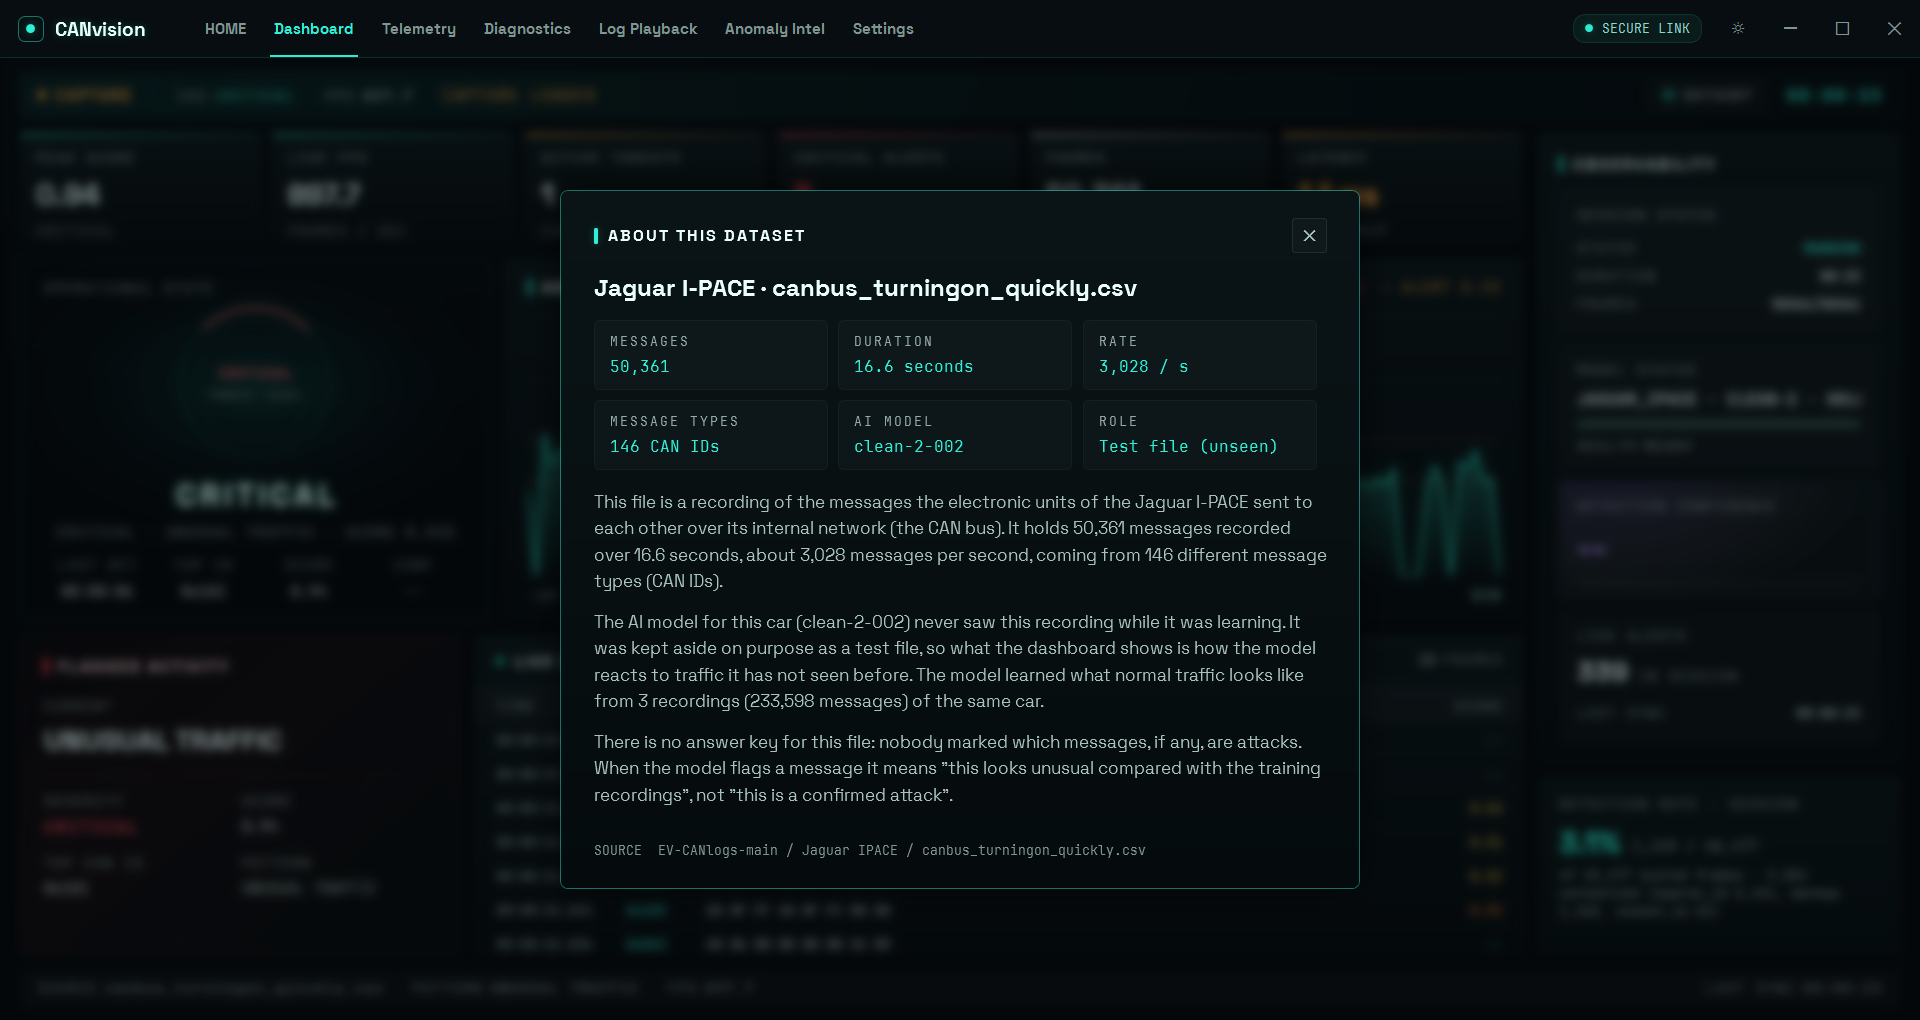
\includegraphics[width=0.9\textwidth]{f02b_dataset_card.png}
\caption{Dataset card of the Jaguar I-PACE holdout recording, open over the Dashboard.}
\label{fig:screen-dataset-card}
\end{figure}

\begin{itemize}
    \item \textbf{Replay log:} The Log Playback screen (Figure~\ref{fig:screen-logplayback}) gives the transport controls and speed, the timeline with the flagged spans, and the detection chart with the threshold of the model.
\end{itemize}

\begin{figure}[H]
\centering
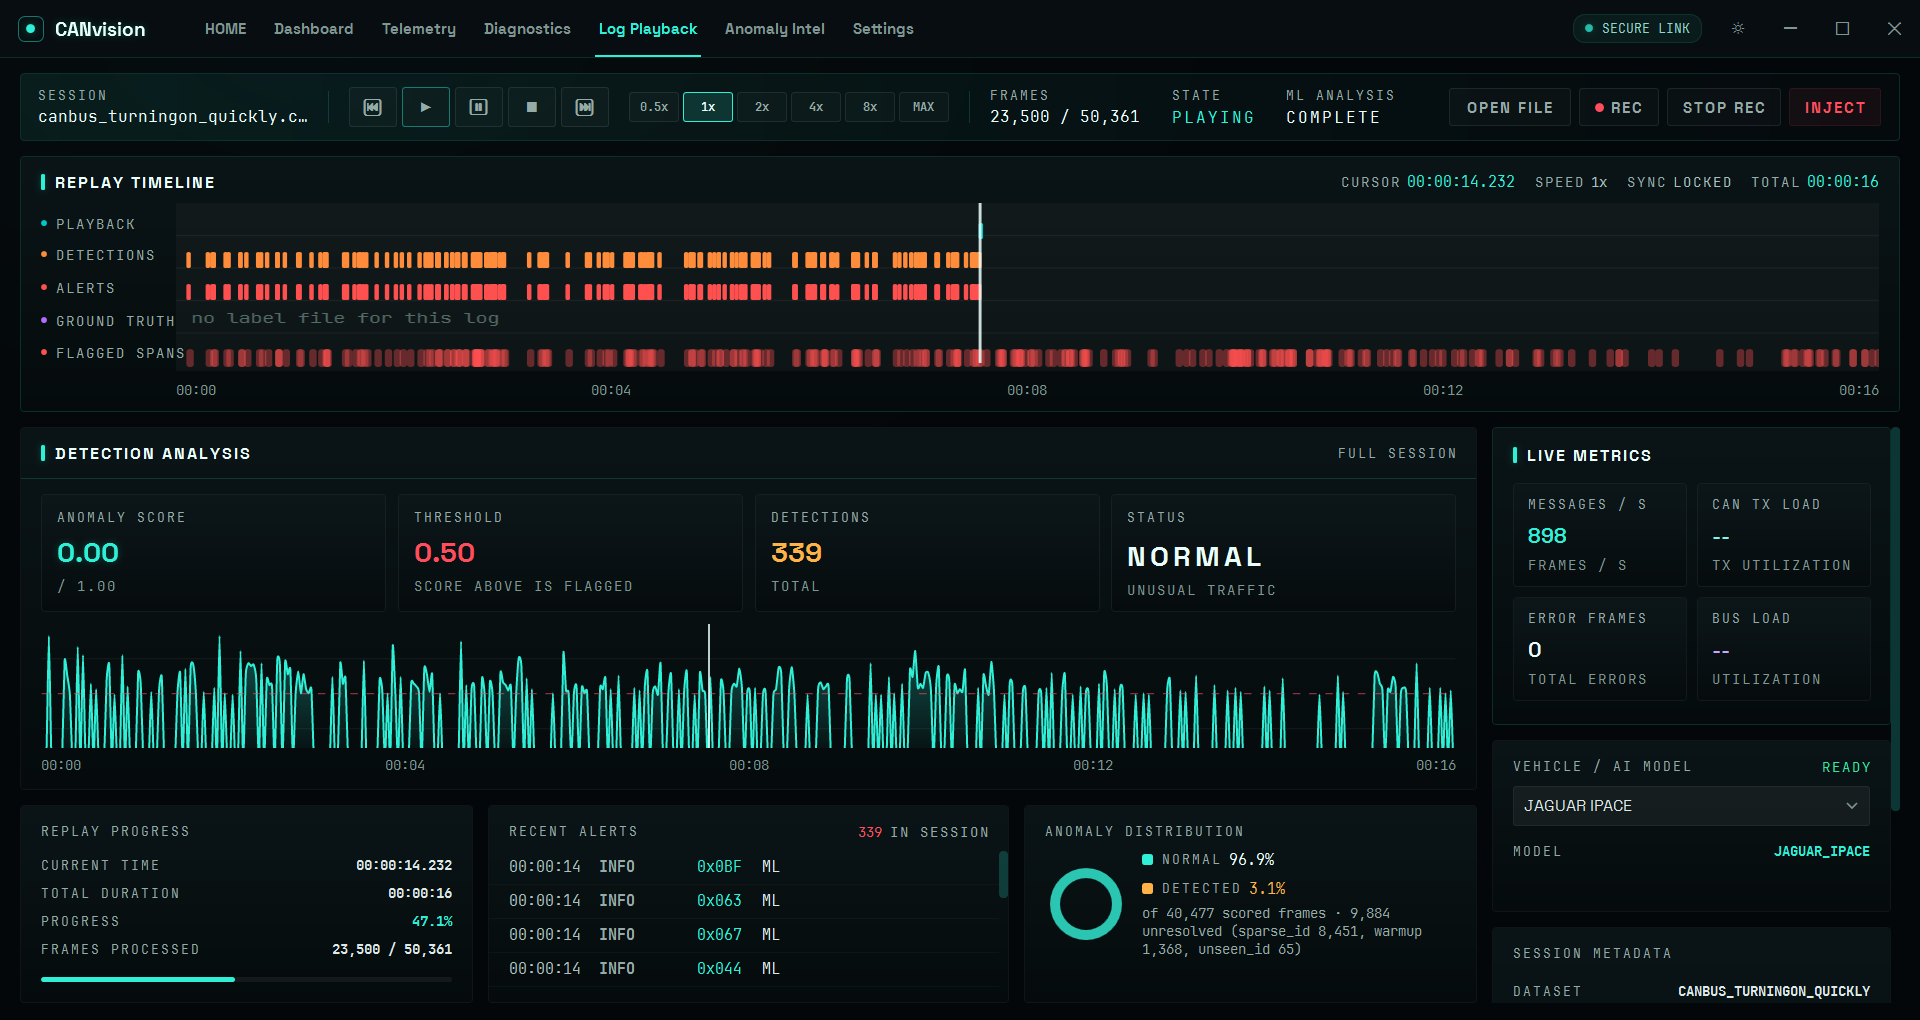
\includegraphics[width=\textwidth]{f07_logplayback.png}
\caption{Log Playback during the replay of the Jaguar I-PACE holdout recording.}
\label{fig:screen-logplayback}
\end{figure}

\Needspace{339pt}% keep the text with its float
\begin{itemize}
    \item \textbf{Review alerts and request an explanation:} Anomaly Intel (Figure~\ref{fig:screen-anomaly-intel}) lists the alerts, shows the signals behind the selected one, and holds the explanation panel. Its alert lists display the offline severities with the labels of Table~\ref{tab:two-paths}.
\end{itemize}

\begin{figure}[H]
\centering
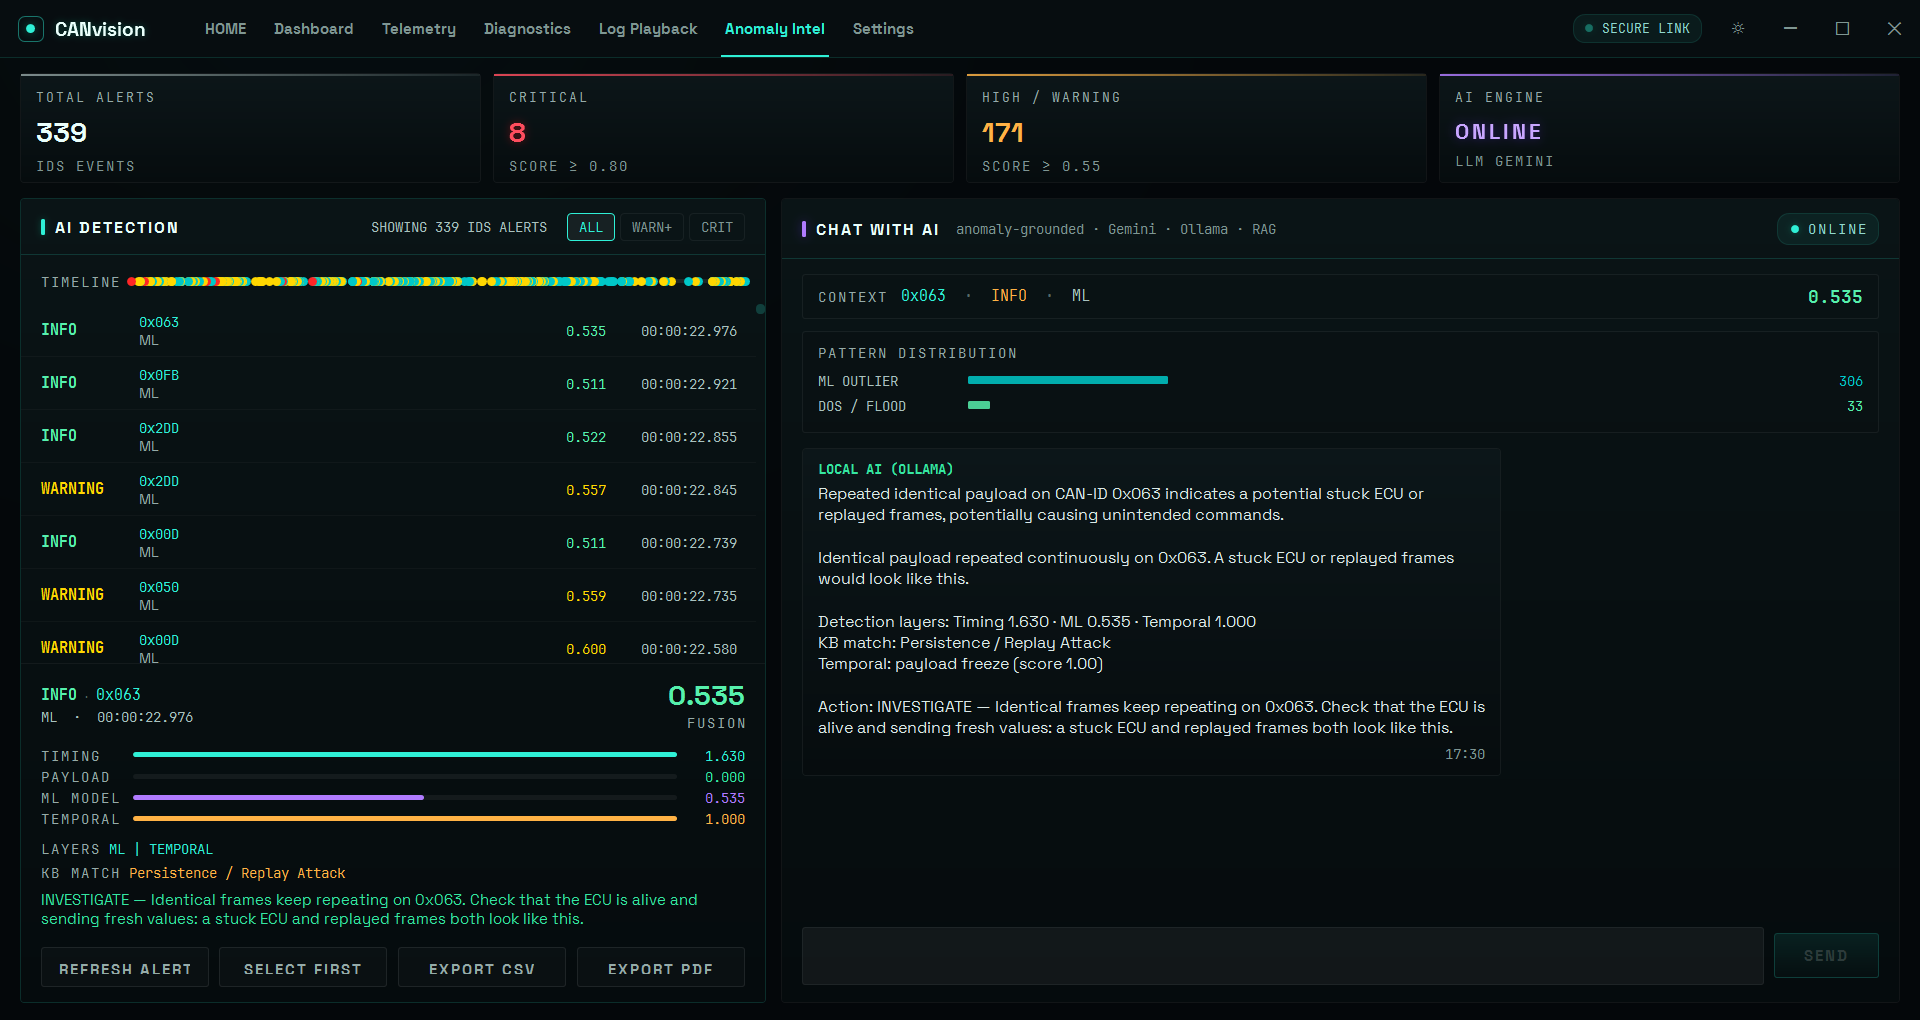
\includegraphics[width=\textwidth]{f08_anomaly_intel.png}
\caption{Anomaly Intel: alert list, signals of the selected alert and explanation panel.}
\label{fig:screen-anomaly-intel}
\end{figure}

\begin{itemize}
    \item \textbf{Export a PDF report:} Anomaly Intel exports the alert list as a PDF report or a \gls{csv} file. The PDF report (Figure~\ref{fig:screen-export-pdf}) gives the session (recording, model and its status, frames analysed, scored, flagged and unresolved), a summary by severity, the identifiers with the most alerts, the alerts in time order, and the explanations requested during the session with the engine that wrote them; for the Jaguar I-PACE analysis it has 13 pages.
\end{itemize}

\begin{figure}[H]
\centering
{\setlength{\fboxsep}{0pt}\setlength{\fboxrule}{0.4pt}\fbox{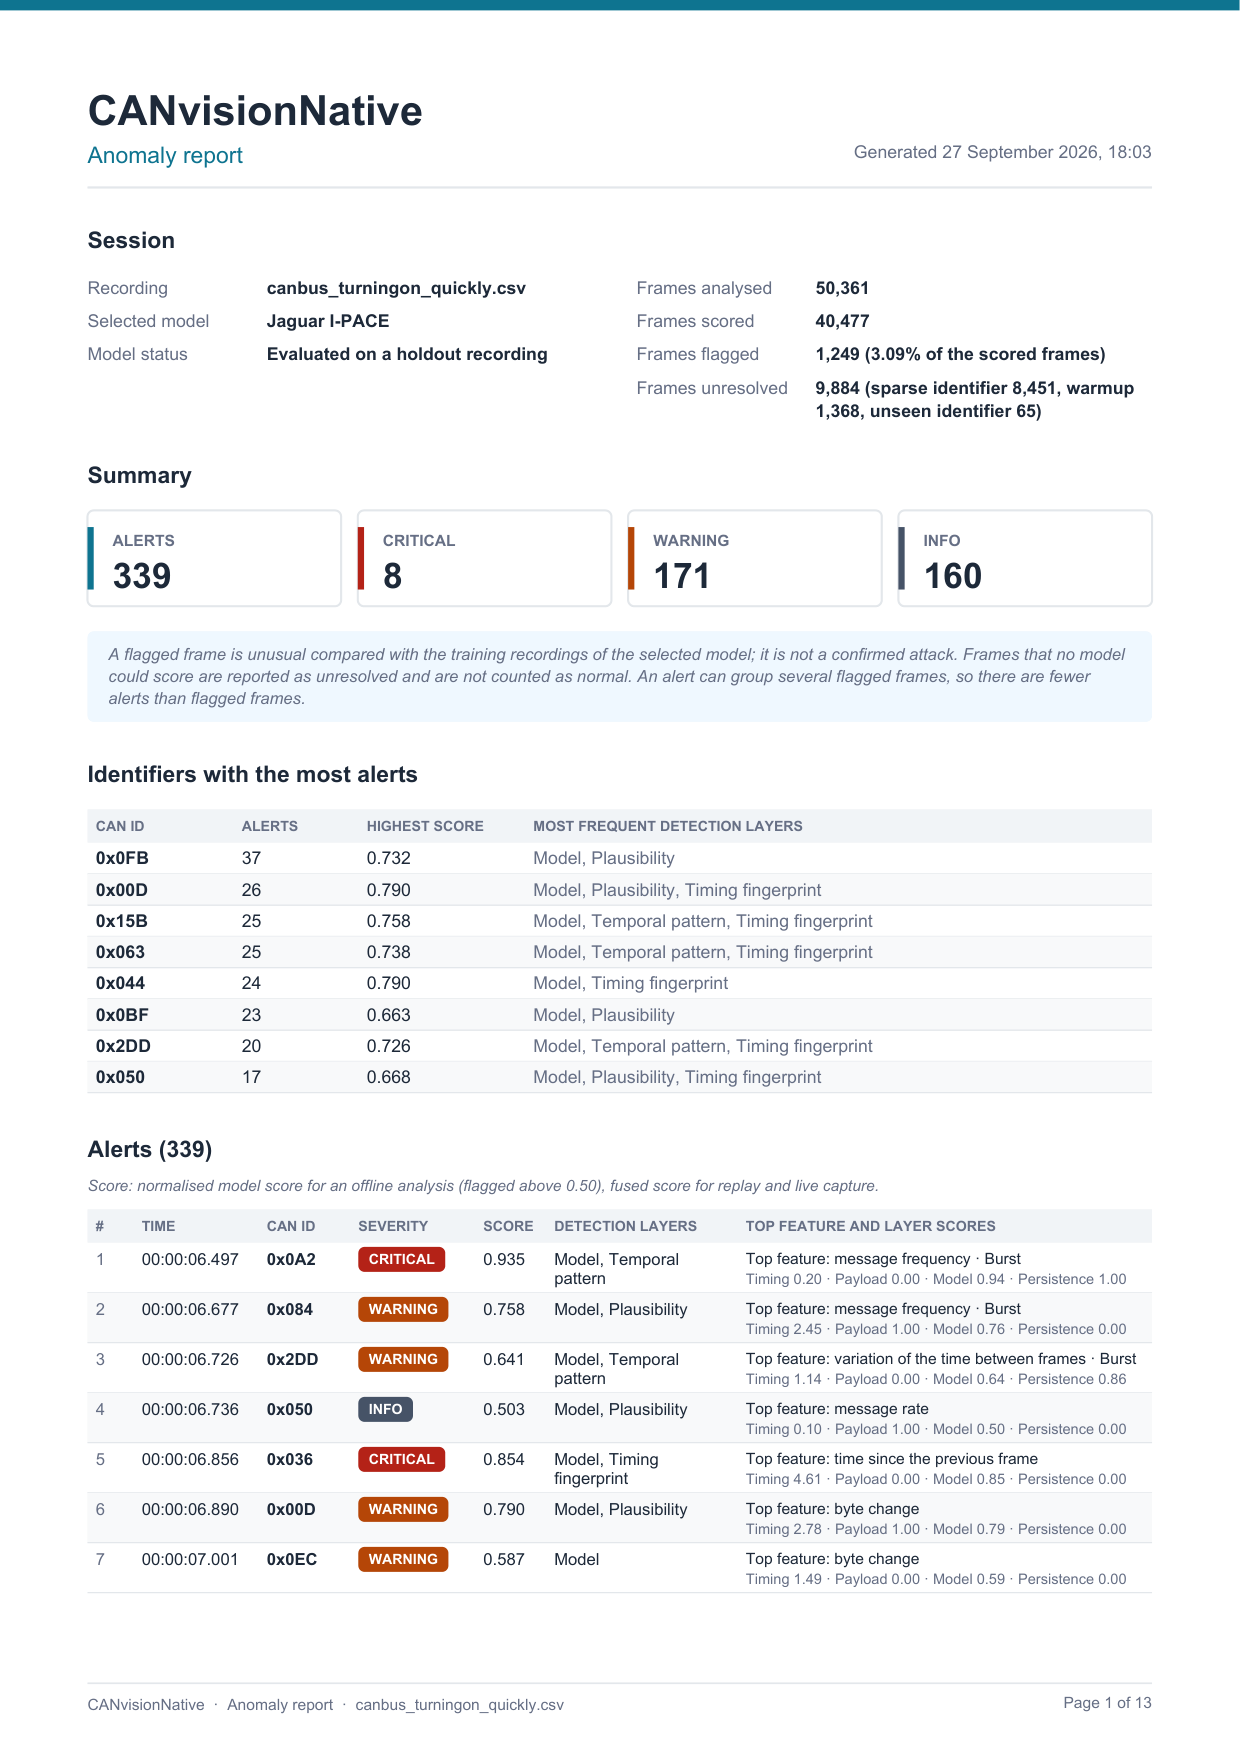
\includegraphics[width=0.62\textwidth]{f10_export_pdf.png}}}
\caption{First page of the PDF report of the Jaguar I-PACE analysis (339 alerts).}
\label{fig:screen-export-pdf}
\end{figure}

\begin{itemize}
    \item \textbf{Export a \gls{csv} file:} The \gls{csv} file (Figure~\ref{fig:screen-export-csv}) has one row per alert, and adds the knowledge base match and the explanation of each alert to the columns of the list.
\end{itemize}

\begin{figure}[H]
\centering
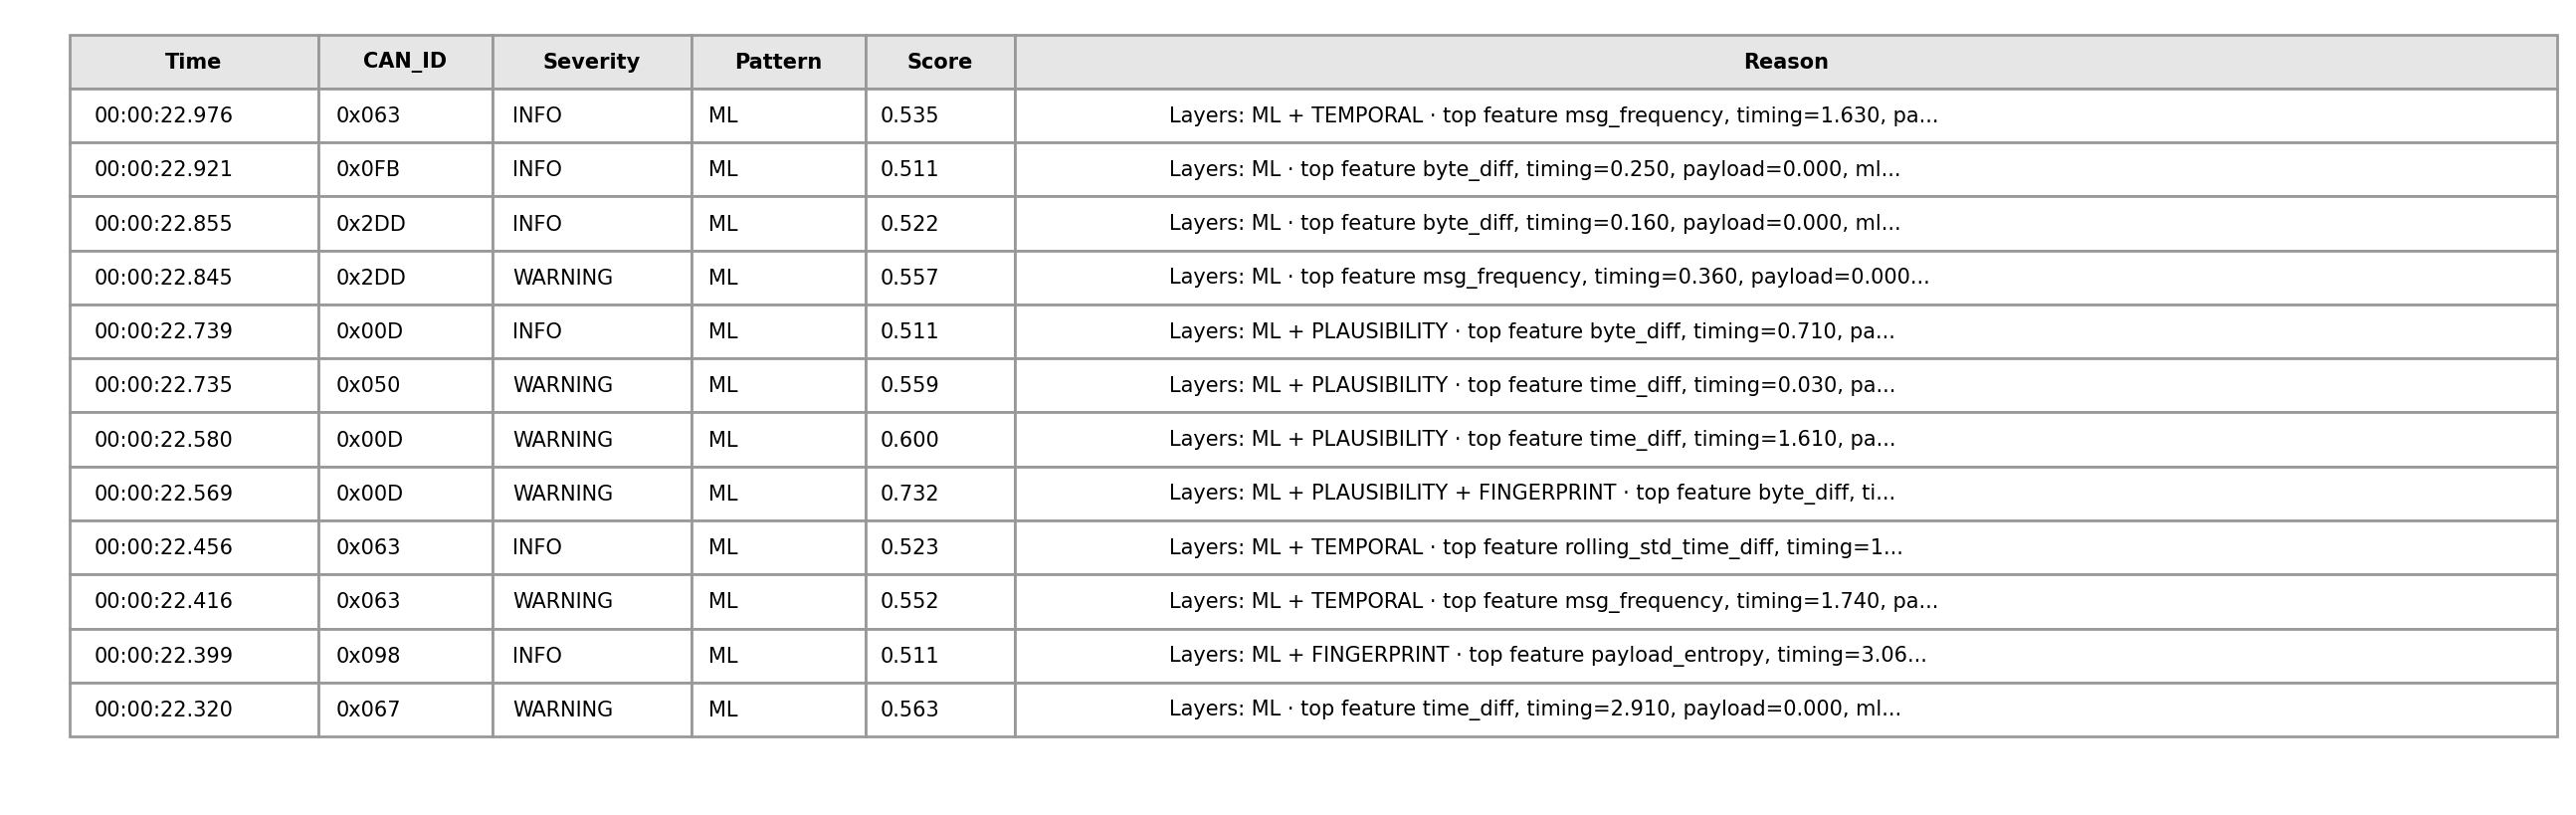
\includegraphics[width=\textwidth]{f09_export_csv.png}
\caption{First rows of the exported \acrshort{csv} file of the same analysis.}
\label{fig:screen-export-csv}
\end{figure}

\begin{itemize}
    \item \textbf{Signals of the capture:} Telemetry (Figure~\ref{fig:screen-telemetry}) shows the signals found in the capture, the live signal monitor and the activity of each identifier. No \gls{dbc} file exists for the Jaguar I-PACE, so the channels are raw payload bytes, labelled as undecoded, as required by FR12. A Diagnostics screen gathers the state of the adapter and the event log of a session.
\end{itemize}

\begin{figure}[H]
\centering
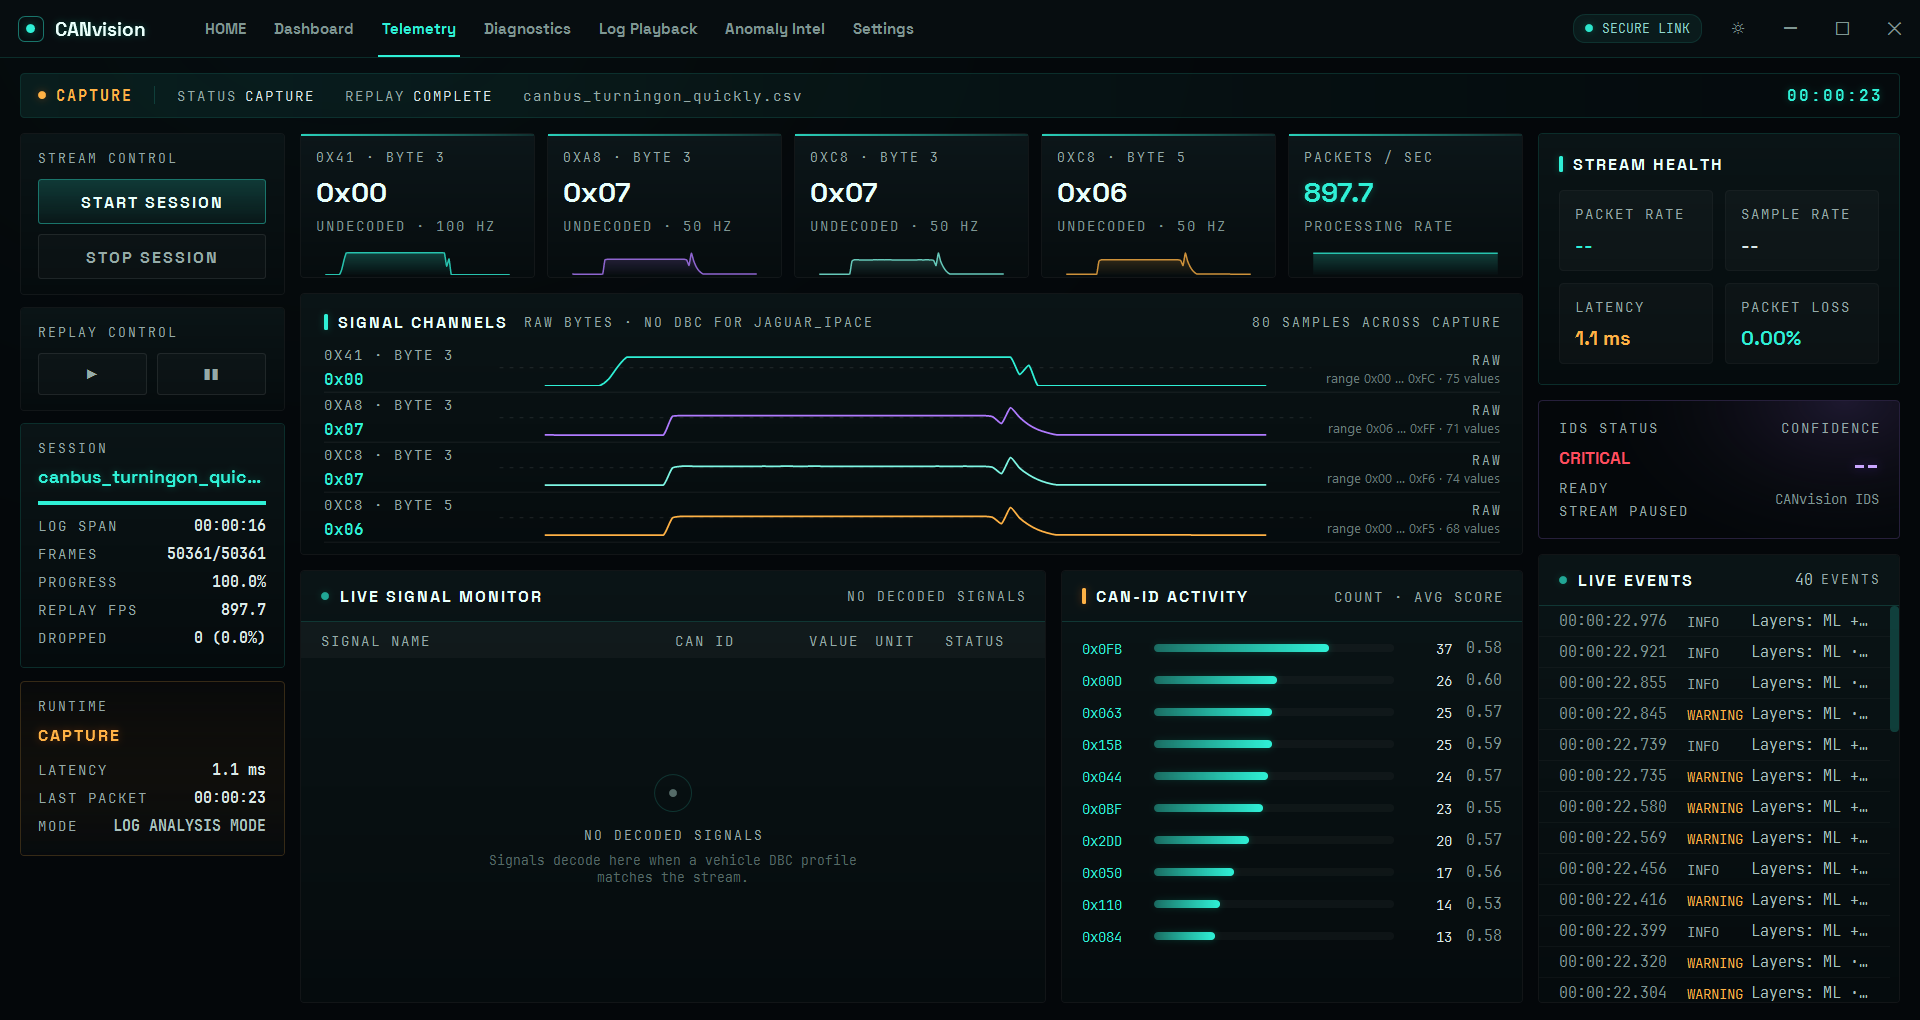
\includegraphics[width=\textwidth]{f03_telemetry.png}
\caption[Telemetry: channels of the Jaguar I-PACE recording.]{Telemetry: channels of the Jaguar I-PACE recording. No \acrshort{dbc} file exists for this vehicle, so the channels are raw payload bytes, marked as undecoded.}
\label{fig:screen-telemetry}
\end{figure}

\begin{itemize}
    \item \textbf{Configure settings:} The Settings screen holds the key of the \gls{llm} provider, the hardware interface (adapter, serial port, bitrate) and an alert threshold, saved locally between sessions. In the current version, this threshold is only stored by the client: it is not sent to the backend, which scores with the values of Table~\ref{tab:two-paths}.
\end{itemize}

\Needspace{690pt}% keep the heading with its float
\section{Test strategy and results}
\label{sec:tests}

\subsection{Test plan}

The same rule applied to every test: a claim had to be backed by reproducible evidence, a defect counted as found only once it could be triggered on demand, and as fixed only once the same test, run again, gave the expected result. Table~\ref{tab:qa-timeline} lists the stages of the validation over the iterations, and Table~\ref{tab:testing-matrix} what each kind of test covered.

\begin{table}[H]
\centering
\footnotesize
\caption{Stages of the validation.}
\label{tab:qa-timeline}
\begin{tabularx}{\textwidth}{|P{4.4cm}|P{2.0cm}|Y|}
\hline
\textbf{Stage} & \textbf{When} & \textbf{Description} \\
\hline
1. Interactive interface audit & Iteration 2 & Exploratory testing of the running application: every screen and every control, actions in the wrong order, destructive actions, resizing and minimising during a replay. \\
\hline
2. Root cause analysis of the alerts & Iteration 2 & Full replay of a one hour Kia EV6 recording, with every alert explained and attributed to a dominant cause. \\
\hline
3. Correction and new validation & Iteration 2 & Each confirmed defect fixed on its own and verified again, then a full run of the corrected pipeline on the same recording. \\
\hline
4. Live capture on the bench rig & Iteration 3 & Frames of the rig read through python-can, then through the hardware layer of the application. \\
\hline
5. Evaluation of the final models & Iteration 4 & Each rebuilt model scored on a complete recording kept out of its training; speed measured; three algorithms compared. \\
\hline
6. End to end test of the release & Transition & The whole application used on a holdout recording, from import to export. \\
\hline
\end{tabularx}
\end{table}

\begin{table}[H]
\centering
\small
\caption{Testing matrix: what was covered, and how.}
\label{tab:testing-matrix}
\begin{tabularx}{\textwidth}{|l|Y|Y|}
\hline
\textbf{Target} & \textbf{Method} & \textbf{Coverage} \\
\hline
Desktop interface & Automation of the running client (clicks, file dialogs, keyboard) and screenshots & Navigation, import, replay controls, actions in the wrong order or repeated \\
\hline
Detection pipeline & Direct calls to the backend \gls{api} and full replays of real recordings & Vehicle selection, scoring, reasons shown to the analyst \\
\hline
Parsers & Small test files per format (\gls{csv}, candump, Vector) and real recordings & Extraction of the frames, byte for byte comparison with a known good output \\
\hline
Final models & Scoring of complete holdout recordings, and checks of each manifest & Flagged rate on new recordings, coverage, consistency of the thresholds \\
\hline
Explanations & Direct \gls{api} calls on two datasets from different vehicles & Correctness per alert, no mixing between sessions or datasets \\
\hline
Live capture & Bench rig, and the virtual bus of python-can in automated tests & Transport of the frames, decoding, alert on an unknown identifier \\
\hline
Export & Manual export and direct inspection of the files & Columns of the \gls{csv} file, rendering and pagination of the PDF \\
\hline
End to end & Full walk through the application (import, analysis, replay, explanation, export) & Integration of every layer, on real recordings \\
\hline
\end{tabularx}
\end{table}

\subsection{Automated tests}

Two automated suites run after every change. The 318 backend tests (pytest) cover the parsers, the manifest checks, the model statuses and refusals, the scoring and the unresolved frames, the threshold calibration, signal discovery, the dataset description, the temporal patterns, the explanation texts and the bench rig profile. The 86 desktop tests (xUnit) cover the import of logs, the \gls{api} contracts, the detection of USB devices, the dataset card, the discovered signals and the PDF report. Both suites pass, and the Release build of the client compiles without warnings.

\subsection{End to end test of the release}
\label{sec:e2e}

Analysing the Jaguar I-PACE holdout file through the application gave the same numbers as the evaluation of Section~\ref{sec:validation-protocol}: 50{,}361 frames, 40{,}477 scored and 1{,}249 flagged (Section~\ref{sec:tour}). This test also revealed display problems, corrected before the screenshots of Section~\ref{sec:tour} were taken. The \gls{csv} exports wrote the scores with the decimal comma of a French Windows installation, which shifted the columns of the file; after the fix, the 339 exported rows all read back with the nine columns of the header. A bus load was shown that was in fact the processing rate of the application divided by twenty. A frequency analysis labelled an identifier sending 0.2 messages per second as a denial of service burst, because its baseline was almost zero. And some explanation texts presented a possible attack as a fact on unlabelled data.

\subsection{Performance}

The offline analysis meets NFR1: the 491{,}969 frames of the Nissan Leaf holdout were analysed in 187 seconds, and the Jaguar I-PACE file in about one minute in the application. The live path processes about 200 to 260 frames per second (Table~\ref{tab:perf-live}), which keeps up with a slow bus such as the one of the Nissan Leaf, but not with buses that carry thousands of frames per second.

\Needspace{385pt}% keep the heading with its float
\section{Requirements traceability}
\label{sec:traceability}

Table~\ref{tab:traceability} links each functional requirement to its implementation and to the evidence that validates it.

\begin{table}[H]
\centering
\footnotesize
\caption{Requirements traceability, from requirement to implementation to validation.}
\label{tab:traceability}
\begin{tabularx}{\textwidth}{|P{1.1cm}|P{6.0cm}|Y|}
\hline
\textbf{Req.} & \textbf{Implemented in} & \textbf{Validated by} \\
\hline
FR1 & Common parser, Section~\ref{sec:impl-parser} & Fix 4, Section~\ref{sec:it2} \\
\hline
FR2 & Vehicle profiles and model selection, Section~\ref{sec:impl-vehicle} & Fix 1, Section~\ref{sec:it2} \\
\hline
FR3 & Replay engine, Section~\ref{sec:impl-replay} & Throughput before and after, Table~\ref{tab:before-after} \\
\hline
FR4 & Detection paths, Section~\ref{sec:design-pipeline}; final models, Section~\ref{sec:impl-feature-eng} & Root cause analysis, Table~\ref{tab:rootcause}; holdout results, Table~\ref{tab:holdout-results} \\
\hline
FR5 & Severity rules, Table~\ref{tab:two-paths} & Severity distribution, Figure~\ref{fig:chart-severity} \\
\hline
FR6 & Explanation engine, Section~\ref{sec:design-ai} & Fix 6, Section~\ref{sec:validation-ai} \\
\hline
FR7 & Exports, Section~\ref{sec:it1} & End to end test, Section~\ref{sec:e2e} \\
\hline
FR8 & Live simulation, Section~\ref{sec:baseline} & Interactive interface audit, Section~\ref{sec:it2} \\
\hline
FR9 & Hardware layer, Section~\ref{sec:impl-hardware} & Bench rig test, Section~\ref{sec:validation-bench}; no vehicle test \\
\hline
FR10 & Session recording, Section~\ref{sec:it1} & Interactive interface audit, Section~\ref{sec:it2} \\
\hline
FR11 & Settings, Section~\ref{sec:tour} & Interactive interface audit, Section~\ref{sec:it2}; the alert threshold is stored but not yet applied \\
\hline
FR12 & Dataset card and signal discovery, Section~\ref{sec:impl-capture} & End to end test, Section~\ref{sec:e2e} \\
\hline
FR13 & Model status and manifest checks, Section~\ref{sec:it4} & Holdout evaluation, Section~\ref{sec:validation-protocol} \\
\hline
\end{tabularx}
\end{table}

Live capture has the weakest evidence: it was tested on a bench rig with synthetic traffic, not on a vehicle.

\section{Deployment and documentation}
\label{sec:deployment}

\subsection{Installation}

The platform is installed on one Windows workstation, as shown in the deployment diagram of Figure~\ref{fig:deployment}. It needs Windows 10 or 11 with .NET Framework 4.8, Python 3.11 or later and Git; a \gls{can} adapter is only needed for live capture. The repository contains a setup guide with the steps below and a troubleshooting section.

\begin{enumerate}
    \item Clone the repository, create a Python virtual environment and install the dependencies of the backend:
\begin{lstlisting}[numbers=none]
python -m venv .venv
.venv\Scripts\activate
pip install -r requirements.txt
\end{lstlisting}
    \item Optionally, give the explanation module a language model: enter a Google Gemini key in the Settings screen of the client, which stores it in the configuration file of the user, or set the variable \code{GOOGLE\_API\_KEY}; or install Ollama and pull a local model, which the backend uses when Gemini is not configured. Without either, the explanations are written by the rule based template.
    \item Start the backend and check that it answers:
\begin{lstlisting}[numbers=none]
python -m uvicorn backend.api.server:app --host 127.0.0.1 --port 8765
curl http://127.0.0.1:8765/health
\end{lstlisting}
    The client also starts the backend by itself when it finds the Python installation.
    \item Start the client, \code{CANvisionNative.exe}. The connection state of the backend is shown in the top right corner of every screen.
\end{enumerate}

\subsection{Model promotion}

New vehicle models are produced and promoted with the commands of the training pipeline (Section~\ref{sec:impl-models}). \code{plan} checks the corpus and prints the split without fitting anything; \code{train} fits a version into the staging folder; \code{validate} checks a staged version; and \code{promote} validates it again and moves it into production, archiving the files it replaces:

\begin{lstlisting}[numbers=none]
python -m backend.ml.training.clean_pipeline plan
python -m backend.ml.training.clean_pipeline train --version <version>
python -m backend.ml.training.clean_pipeline validate --version <version>
python -m backend.ml.training.clean_pipeline promote --version <version>
\end{lstlisting}

A held back vehicle is refused by the promotion step, and the model files in production are versioned with Git LFS.

\subsection{User guide}

Table~\ref{tab:user-guide} gives the main tasks of the analyst and how to perform them.

\begin{table}[H]
\centering
\small
\caption{User guide: main tasks.}
\label{tab:user-guide}
\begin{tabularx}{\textwidth}{|P{3.2cm}|Y|}
\hline
\textbf{Task} & \textbf{How} \\
\hline
Analyse a recording & On Home, import a log file, choose the vehicle model (its status is shown next to it) and run the analysis. The results open on the Dashboard. \\
\hline
Check the dataset & On the Dashboard, open the Dataset card to see the size of the recording and whether the model was trained or tested on it. \\
\hline
Replay a recording & In Log Playback, choose a speed and play; the flagged spans and the alerts appear on the timeline. \\
\hline
Explain an alert & In Anomaly Intel, select an alert; the explanation panel shows the summary, the likely cause, the recommendation and the engine that wrote them. \\
\hline
Export the results & In Anomaly Intel, export the alert list as a PDF report or a \gls{csv} file. \\
\hline
Watch a live bus & Plug in a supported \gls{can} adapter, start a live session on Home, choose the interface, port, bitrate and vehicle model, and connect. \\
\hline
Change the settings & In Settings, set the key of the language model, the hardware interface and the alert threshold, then save. \\
\hline
\end{tabularx}
\end{table}

\section{Stability scope and limitations}
\label{sec:limitations}

Within the scope of this validation, we consider the software stable:

\begin{itemize}
    \item \textbf{All known defects are fixed and verified} with direct evidence.
    \item \textbf{Every model in production was evaluated} on a recording it never saw, and the application shows the status of every model.
    \item \textbf{No silent fallback remains:} Unscored frames are reported with their reason, and a model that may not be used is refused, not replaced.
    \item \textbf{The frame by frame paths share one engine}, and replay and offline analysis share one parser; the offline analysis turns scores into alerts differently (Table~\ref{tab:two-paths}).
    \item \textbf{The pipeline was checked end to end} on real recordings, from import to export.
\end{itemize}

This scope has limits, which we state plainly. It is not a production, safety or security certification, and it does not cover deployment in a vehicle. Live capture was tested only on a bench rig with synthetic traffic, since no compatible vehicle was available, and the run on the physical rig has not been repeated after the last corrections. The final models were evaluated on recordings without attack labels, so we can report flagged rates but no detection rate, precision or recall; we did not evaluate the final models on the labelled attack recordings of public datasets. The live path is too slow for buses above about 260 frames per second. The weights and thresholds of the fused score are fixed configuration values whose effect was not evaluated separately, and the alert threshold shown in the Settings screen is stored but not yet applied to scoring. The coverage of some vehicles is incomplete: on the Jaguar I-PACE, about a fifth of the frames cannot be scored, mostly because they belong to identifiers too rare to have a model. Each vehicle was evaluated on one holdout recording, which says more about that recording than about every driving situation. Finally, the explanations may cite a similar past case, and this history is kept across sessions on purpose, so an analyst who compares two unrelated vehicles may see a past case from the other vehicle.

\section{Conclusion}

The transition phase delivered a release whose screens cover every use case, checked by automated tests and by an end to end test on a recording the models never saw. Every functional requirement is traced to its implementation and its evidence, the platform comes with an installation procedure, a model promotion procedure and a user guide, and its limits are measured and stated.
